% Options for packages loaded elsewhere
\PassOptionsToPackage{unicode}{hyperref}
\PassOptionsToPackage{hyphens}{url}
%
\documentclass[
]{book}
\usepackage{lmodern}
\usepackage{amsmath}
\usepackage{ifxetex,ifluatex}
\ifnum 0\ifxetex 1\fi\ifluatex 1\fi=0 % if pdftex
  \usepackage[T1]{fontenc}
  \usepackage[utf8]{inputenc}
  \usepackage{textcomp} % provide euro and other symbols
  \usepackage{amssymb}
\else % if luatex or xetex
  \usepackage{unicode-math}
  \defaultfontfeatures{Scale=MatchLowercase}
  \defaultfontfeatures[\rmfamily]{Ligatures=TeX,Scale=1}
\fi
% Use upquote if available, for straight quotes in verbatim environments
\IfFileExists{upquote.sty}{\usepackage{upquote}}{}
\IfFileExists{microtype.sty}{% use microtype if available
  \usepackage[]{microtype}
  \UseMicrotypeSet[protrusion]{basicmath} % disable protrusion for tt fonts
}{}
\makeatletter
\@ifundefined{KOMAClassName}{% if non-KOMA class
  \IfFileExists{parskip.sty}{%
    \usepackage{parskip}
  }{% else
    \setlength{\parindent}{0pt}
    \setlength{\parskip}{6pt plus 2pt minus 1pt}}
}{% if KOMA class
  \KOMAoptions{parskip=half}}
\makeatother
\usepackage{xcolor}
\IfFileExists{xurl.sty}{\usepackage{xurl}}{} % add URL line breaks if available
\IfFileExists{bookmark.sty}{\usepackage{bookmark}}{\usepackage{hyperref}}
\hypersetup{
  pdftitle={Transparencia y Reproducibilidad en Investigación Social},
  pdfauthor={Julio Iturra y Martín Venegas},
  hidelinks,
  pdfcreator={LaTeX via pandoc}}
\urlstyle{same} % disable monospaced font for URLs
\usepackage{longtable,booktabs}
% Correct order of tables after \paragraph or \subparagraph
\usepackage{etoolbox}
\makeatletter
\patchcmd\longtable{\par}{\if@noskipsec\mbox{}\fi\par}{}{}
\makeatother
% Allow footnotes in longtable head/foot
\IfFileExists{footnotehyper.sty}{\usepackage{footnotehyper}}{\usepackage{footnote}}
\makesavenoteenv{longtable}
\usepackage{graphicx}
\makeatletter
\def\maxwidth{\ifdim\Gin@nat@width>\linewidth\linewidth\else\Gin@nat@width\fi}
\def\maxheight{\ifdim\Gin@nat@height>\textheight\textheight\else\Gin@nat@height\fi}
\makeatother
% Scale images if necessary, so that they will not overflow the page
% margins by default, and it is still possible to overwrite the defaults
% using explicit options in \includegraphics[width, height, ...]{}
\setkeys{Gin}{width=\maxwidth,height=\maxheight,keepaspectratio}
% Set default figure placement to htbp
\makeatletter
\def\fps@figure{htbp}
\makeatother
\setlength{\emergencystretch}{3em} % prevent overfull lines
\providecommand{\tightlist}{%
  \setlength{\itemsep}{0pt}\setlength{\parskip}{0pt}}
\setcounter{secnumdepth}{5}
\usepackage{booktabs}
\usepackage{booktabs}
\usepackage{longtable}
\usepackage{array}
\usepackage{multirow}
\usepackage{wrapfig}
\usepackage{float}
\usepackage{colortbl}
\usepackage{pdflscape}
\usepackage{tabu}
\usepackage{threeparttable}
\usepackage{threeparttablex}
\usepackage[normalem]{ulem}
\usepackage{makecell}
\usepackage{xcolor}
\ifluatex
  \usepackage{selnolig}  % disable illegal ligatures
\fi
\usepackage[]{natbib}
\bibliographystyle{apalike}

\title{Transparencia y Reproducibilidad en Investigación Social}
\author{Julio Iturra y Martín Venegas}
\date{2021-07-27}

\begin{document}
\maketitle

{
\setcounter{tocdepth}{1}
\tableofcontents
}
\hypertarget{intro}{%
\chapter{Introducción}\label{intro}}

Imagine que usted es un chef, y como tal, disfruta enormemente de las artes culinarias. Como amante de la cocina, cada vez que alguna celebración especial se avecina, es tradición preparar sus mejores recetas para sus invitados. Sin embargo, en esta ocasión, la celebración se llevará a cabo en un restaurante, lo cual implica que la preparación de la comida no depende de usted. Con bastantes dudas, usted accede, teniendo en mente la siguiente pregunta: ¿Cómo puedo tener certeza de que se seguirán los procedimientos adecuados para que la preparación sea de calidad? Pues, estimado lector, es esta la pregunta que subyace a todo el proceso que engloba al conocimiento científico.

La ciencia, al igual que la cocina, no se trata solamente de los productos. Una preparación no aparece por generación espontánea, sino que requiere el seguimiento riguroso de una receta, donde usamos los ingredientes, las cantidades y tiempos de cocción adecuados. Esta receta no solo contribuye a la preparación de la comida, sino que hace posible que dicho plato pueda ser \textbf{reproducido} cada vez que se lo desee, garantizando el mismo resultado. Entonces, como buen chef, la respuesta a la pregunta no es tan compleja: necesitamos ser capaces de evaluar el proceso de elaboración de la comida para asegurarnos de que es el adecuado. Dicho de otro modo, el proceso de preparación debe ser \textbf{transparente} y estar abierto al escrutinio de otros cocineros expertos, como también para quienes estén adentrándose en la cocina. En el caso de la comida, que el restaurante cuente con una cocina abierta o construida en torno a ventanales bastaría para lograr este objetivo. Sin embargo, dentro del campo de la ciencia ¿cómo logramos que el proceso de producción del conocimiento científico esté abierto al escrutinio público?

Esta pregunta puede ser algo engañosa ¿acaso los procesos de investigación en la ciencia no están ya abiertos al escrutinio público? La narrativa actual pareciese sugerir que no. En el último tiempo ha primado el diagnostico de que la ciencia está viviendo una crisis, donde polémicas situaciones de malas prácticas académicas han salido a la luz. Un ejemplo de estas malas prácticas es el falseamiento de datos. Uno de los casos más emblemáticos es el de Diderik Stapel, una figura académica con alto prestigio en el campo de la psicología social a quién se le acusó y confirmó de falseamiento de datos. Más de 10 años de investigación y 150 artículos -algunos de ellos en las revistas más prestigiosas- fueron puestos en duda a raíz de las malas prácticas de Stapel. Así también el trabajo de muchos colegas y estudiantes fue desacreditado. El caso del ex doctor Stapel acabó en la revocación de su doctorado, la retracción de 58 artículos de investigación y, prácticamente, el fin de su carrera académica.

Casos como el de Diderik Stapel existen muchos \citep[ver][]{abrilruiz_Manzanas_2019}, sin embargo, no son las prácticas más recurrentes. Dentro de la investigación científica existen una serie de prácticas que caen en un terreno gris cuando se trata de su evaluación ética, estas son las llamadas \emph{prácticas cuestionables de investigación}. La preocupación dentro de la comunidad científica es que la acumulación y la poca fiscalización de estas prácticas lleven a una ciencia poco transparente, con dificultad en torno a la reproducibilidad de los análisis y de sus resultados, y que a la larga se pierda la confianza en el quehacer científico.

La perdida de la confianza en el quehacer científico afecta el objetivo de las ciencias sociales. Generalmente se tiene la concepción de que es parte de las tareas de los científicos sociales el contribuir al bienestar de la sociedad por la vía de las herramientas de investigación. Esta es la noción de las ciencias sociales como un bien público \citep{thibodeaux_Production_2016}. Bajo esa idea, los efectos de una crisis de credibilidad tienen dos posibles efectos concretos en las ciencias sociales. Primero, la falta de credibilidad podría afectar la confianza en los hallazgos y en las disciplinas que componen las ciencias sociales. Ya existe evidencia sobre un incremento de desconfianza hacia los científicos en países como Estados Unidos \citep{motta_Dynamics_2018} y sumarle una crisis de la ciencia a esa situación solo generaría un ambiente mucho más complejo. Segundo, y estrechamente relacionado a lo anterior, una perdida de credibilidad en la ciencia podría impactar en la elaboración de políticas sociales, mal orientando las prioridades y los recursos del país. Si se quieren evitar estas situaciones, es necesario tomar cartas en el asunto y orientar los esfuerzos a devolverle la credibilidad a las ciencias sociales.

Este manual busca contribuir a una ciencia social más creíble, basándose en el marco de la ciencia abierta. La ciencia abierta se entiende como:

\begin{quote}
``\ldots la práctica de la ciencia de manera que otros puedan colaborar y contribuir, donde los datos de la investigación, las notas de laboratorio y otros procesos de investigación estén disponibles libremente, en términos que permitan la reutilización, redistribución y reproducción de la investigación y sus datos y métodos subyacentes''. (FORSTER, Open Science Teaching Resource)
\end{quote}

Dentro de la ciencia abierta, nos centraremos en dos conceptos: transparencia y reproducibilidad. Si seguimos la metáfora de la cocina que planteamos en un principio, la transparencia y la reproducibilidad son dos conceptos similares, pero no idénticos. La transparencia implicaría la posibilidad de evaluar y poner en discusión la receta y la ejecución de la misma. En cambio, la reproducibilidad apuntaría a que la receta sea lo suficientemente clara y precisa para que el mismo plato, con el mismo sabor, pueda ser preparado por cualquier persona que contase con los ingredientes y recursos necesarios. En el campo de las ciencias, esta distinción la hacemos entre: 1) la transparencia de los procesos de producción científica (e.g.~transparentar el plan de análisis) y 2) la reproducibilidad de los análisis en los artículos (e.g.~código de procesamiento y análisis de datos permite reproducir el artículo). Este manual estará estructurado en torno a estas dos conceptos.

Relacionado al primer concepto (transparencia), haremos un barrido un tanto más detallado sobre la crisis de la reproducibilidad que aquí hemos mencionado brevemente. Ahondaremos en los factores que contribuyen a su reproducción, a las razones éticas por el cuales es necesario hacer un cambio y en las recomendaciones que se pueden seguir para adoptar ciertos principios de transparencia. En el caso del segundo concepto (reproducibilidad), nos centraremos en los análisis reproducibles, teniendo un carácter mucho más práctico. Presentaremos las distintas consideraciones que hay que tener para que un análisis sea fácilmente reproducible, desde tipos de flujos de trabajo hasta herramientas específicas que faciliten la reproducibilidad de los análisis.

Estimado investigador o investigadora de las ciencias sociales, este documento va dirigido a usted. Independiente de su disciplina, de su trayectoria académica o de su conocimiento previo con respecto a estas temáticas, en este manual tenemos dos simples objetivos. El primero es que usted pueda convencerse de que, efectivamente, es necesario dar un giro en la forma que hacemos ciencia actualmente y que la adopción de prácticas relacionadas a la ciencia abierta son el primer paso en ese giro. El segundo es poder instruirlo en esa adopción de prácticas, particularmente en lo que respecta a la transparencia y reproducibilidad. Al final de este manual, usted será capaz tanto de argumentar por qué la transparencia y la reproducibilidad son un paso importante en el avance de las ciencia sociales, así como también contará con una serie de herramientas para llevar esto al quehacer académico del día a día.

\hypertarget{transparencia}{%
\chapter{Transparencia}\label{transparencia}}

Esta sección tratará sobre la transaprencia en la investigación cientifica, haciendo enfásis en las ciencias sociales. Nuestro objetivo es poder comunicar de forma clara y concisa tres puntos: a) qué es la transparencia, b) por qué la necesitamos y c) cómo podemos adoptarla. En esta sección profundizaremos en los dos primer puntos. Respecto al tercer punto, entregaremos algunos consejos y recomendaciones que se han dado en la literatura, para después, en la siguiente sección, profundizar en torno a las herramientas que nos permitirían adoptar la transparencia. La tónica de este escrito es la práctica, es decir; todo lo que presentemos acá tiene la finalidad de servir de camino para poder aprender y aprehender herramientas que promueven la transparencia. Dicho esto, comenzemos con los dos primeros puntos.

\hypertarget{quuxe9-es-la-transparencia-un-concepto-multidimensional}{%
\section{¿Qué es la transparencia? Un concepto multidimensional}\label{quuxe9-es-la-transparencia-un-concepto-multidimensional}}

Nuestro punto de partida es que la transparencia es un concepto amplio y multidimensional. Por eso, antes de adentrarnos en sus dimensiones, comencemos con una definición de diccionario. Según la Real Academia Española la transparencia es la cualidad de un cuerpo que permite ver a travez de él. Un ejemplo para llevar esta definición a la práctica es el vidrio de una ventana. La transparencia del vidrio nos permite ver con claridad lo que está el otro lado, como por ejemplo un paisaje. No obstante, ¿qué ocurre cuándo la transparencia del vidrio se va perdiendo? La respuesta es simple, pero potente: la claridad con la que veíamos el paisaje se va difuminando. Esta perdida de claridad puede dar como resultado que nuestra observación del paisaje se torne ambigua y erronea, o dicho de otro modo, cada vez será más dificil analizar el paisaje. Desde este ejemplo se podria plantear un simil con la ciencia; el paisaje equivale al proceso de producción cientifica, y el vidrio representa la claridad con la que podemos analizar este proceso. De esta manera, la base de la idea de transparencia es que permite analizar con claridad un fenomeno, una situación, o en este caso, un proceso.

¿Qué implica un proceso cientifico transparente? Ya existen algunas respuestas a esta pregunta. Por ejemplo, \citet{breznau_Does_2021} entiende la transparencia como una forma en que los investigadores pueden revelar el proceso, ideas y materiales que sustentan un argumento o una teoría, con tal de contribuir a una comunidad científica más ética. Otra perspectiva es la de \citet{aczel_consensusbased_2020}, quienes proponen a la transparencia como un principio que permite evaluar y reproducir los hallazgos científicos, así como también a sintetizar investigaciones y contribuir a la ejecución de metanálisis. \citet{klein_Practical_2018} proponen que la credibilidad de los productos cientificos dependen de la transparencia en la que se basan, y que, en consecuencia, avanzar hacia la transparencia simplemente significa adoptar ciertas prácticas de gestión de la investigación que la hagan menos propensa a errores y más reproducibles. Estas perspectivas son una primera aproximación a las implicancias de un proceso cientifico transparente, no obstante, no representan una presentación exhaustiva del concepto.

Volvamos a nuestro planteamiento incial: la transparencia es un concepto multidimensional. Para abarcar las múltuiples formas que puede adoptar, nos basamos en la taxonomía de \citet{elliott_Taxonomy_2020}. La taxonomía se estructura en torno a cuatro preguntas: ¿por qué?, ¿quienes? ¿qué? y ¿cómo? Cada una de estas preguntas tiene al menos una dimensión asociada. La primera pregunta (\emph{¿por qué?}) se refiere a los propósitos por los cuales es necesario adoptar la transparencia; la segunda pregunta (\emph{¿quienes?}) apunta a la audiencia que está recibiendo la información; la tercera pregunta (\emph{¿qué?}) hace alusión al contenido qué es transparentado y la cuarta pregunta (\emph{¿cómo?}) consiste en cuatro dimensiones distintas sobre cómo adoptar la transparencia: actores, mecanismos, tiempo y lugar. También, la taxonomía propone una dimensión sobre los peligros que podrían afectar a las iniciativas que busquen promover la transparencia.. Una representación gráfica puede verse en la Figura N° \ref{fig:taxonomy}.

\begin{figure}[H]

{\centering 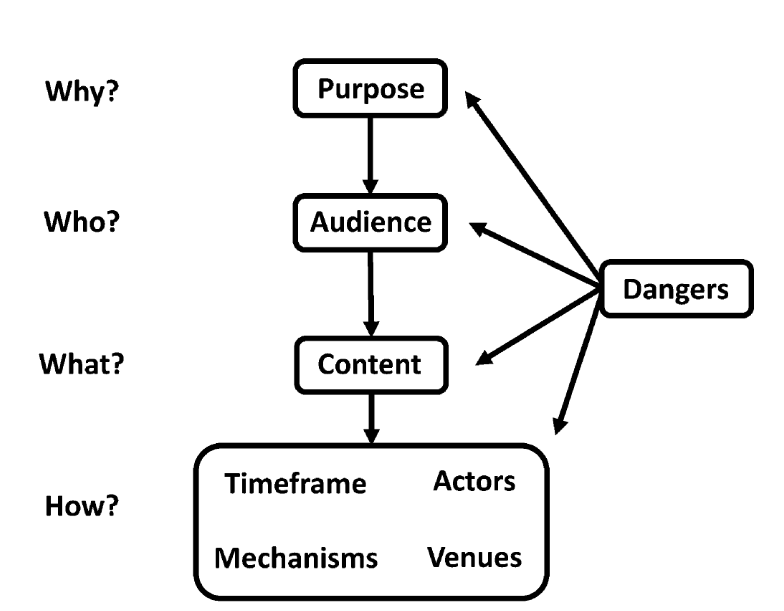
\includegraphics[width=1\linewidth]{docs/images/taxonomy} 

}

\caption{Taxonomía de Transparencia}\label{fig:taxonomy}
\end{figure}

Para comprender mejor la taxonomía la Tabla N° \ref{tab:tabtax} presenta una versión detallada de cada dimensión en conjunto a una lista no exhaustiva de variaciones. Por ejemplo, la dimensión del propósito sintetiza varios de los puntos que ya se han señalado en la literatura sobre ciencia abierta: la transparencia contribuye a formar una ciencia más replicable, facilita la interacción crítica, facilita el reanalisis de resultados, entre otros. La mayoría de estos propositos están estrechamente relacionados con el horizonte de una ciencia con mayor credibilidad, cuestión que profundizarmeos en breve. Dentro de las dimensiones restantes, existe una en particular que queremos recalcar: los contenidos. Aquí, los distintos contenidos que pueden ser transparentados van desde cosas complejas como los juicios de valor o factores que podrían influencias las interpretaciones de resultados, hasta lo más concreto como datos, métodos y materiales, o en otras palabras, el diseño de investigación. Como podemos ver, la transparencia abarca varias dimensiones, sin embargo, a fin de mantener un documento simple y práctico, esta sección apuntará especificamente a la promoción de la transparencia del diseño de investigación.

\begin{table}[!h]

\caption{\label{tab:tabtax}Variaciones por cada dimensión de transparencia}
\centering
\fontsize{10}{12}\selectfont
\begin{tabu} to \linewidth {>{\raggedright\arraybackslash}p{5 cm}>{\raggedright\arraybackslash}p{5 cm}}
\toprule
Dimensión & Variaciones\\
\midrule
 & Facilitar el reanalisis de los resultados\\
\cmidrule{2-2}
 & Hacer a la ciencia más replicable\\
\cmidrule{2-2}
 & Promover la innovación\\
\cmidrule{2-2}
 & Mantener la rendición de cuentas de los expertos\\
\cmidrule{2-2}
 & Facilitar la interacción crítica\\
\cmidrule{2-2}
 & Promover el desarrollo de política pública de alta calidad\\
\cmidrule{2-2}
 & Permitir al público tomar decisiones de acuerdo a sus valores\\
\cmidrule{2-2}
\multirow{-8}{5 cm}{\raggedright\arraybackslash Proposito} & Promover la integridad\\
\cmidrule{1-2}
 & Datos, métodos, código y materiales\\
\cmidrule{2-2}
 & Interpretaciones de los datos, metodos, y codigos para no especialistas\\
\cmidrule{2-2}
 & Juicios de valor, factores que los influencian o sus implicancias\\
\cmidrule{2-2}
\multirow{-4}{5 cm}{\raggedright\arraybackslash Contenido} & Deliberaciones que subyacen a los reportes\\
\cmidrule{1-2}
 & Cientificos que desarrollaron la investigación\\
\cmidrule{2-2}
 & Otros científicos de la misma disciplina u otras\\
\cmidrule{2-2}
 & Periodistas\\
\cmidrule{2-2}
 & Sociedades cientificas\\
\cmidrule{2-2}
 & Agencias gubernamentales\\
\cmidrule{2-2}
\multirow{-6}{5 cm}{\raggedright\arraybackslash Actores} & Organizaciones no gubernamentales y de la sociedad civil\\
\cmidrule{1-2}
 & Comunicación desde los cientificos (oral o escrita, incluyendo las redes sociales)\\
\cmidrule{2-2}
 & Registros o repositorios\\
\cmidrule{2-2}
 & Divulgación cientifica\\
\cmidrule{2-2}
 & Reportes de agencias gubernamentales\\
\cmidrule{2-2}
\multirow{-5}{5 cm}{\raggedright\arraybackslash Espacios} & Reportes de agencias no gubernamentales o grupos de la comunidad\\
\cmidrule{1-2}
 & Cientificos haciendo la investigación\\
\cmidrule{2-2}
 & Otros cientificos\\
\cmidrule{2-2}
 & Desarrolladores de política pública\\
\cmidrule{2-2}
 & Políticos\\
\cmidrule{2-2}
 & Periodistas\\
\cmidrule{2-2}
 & Grupos de interés\\
\cmidrule{2-2}
\multirow{-7}{5 cm}{\raggedright\arraybackslash Audiencia} & Público general\\
\cmidrule{1-2}
 & Antes de que la investigación comience\\
\cmidrule{2-2}
 & Durante el proceso de investigación\\
\cmidrule{2-2}
 & Inmediatamente después de que los datos fueron recolerados\\
\cmidrule{2-2}
 & Despés de la  publicación\\
\cmidrule{2-2}
\multirow{-5}{5 cm}{\raggedright\arraybackslash Marco temporal} & Durante o después de las revisiones o el análisis de la investigación\\
\cmidrule{1-2}
 & Discusiones entre cientificos (orales o escritas)\\
\cmidrule{2-2}
 & Colaboraciones interdisciplinares\\
\cmidrule{2-2}
 & Colaboraciones con miembros de la comunidad\\
\cmidrule{2-2}
 & Organos asesores gubernamentales y otras iniciativas\\
\cmidrule{2-2}
\multirow{-5}{5 cm}{\raggedright\arraybackslash Mecanismos} & Procedimientos contradictorios (e.g. cortes cientificas)\\
\cmidrule{1-2}
 & Desperdiciar recursos escasos\\
\cmidrule{2-2}
 & Ralentizar a la ciencia\\
\cmidrule{2-2}
 & Dañas compañias\\
\cmidrule{2-2}
 & Violación de privacidad\\
\cmidrule{2-2}
 & Generación de escepticismo inapropiado\\
\cmidrule{2-2}
 & Crear un falso sentido de confianza\\
\cmidrule{2-2}
 & Causar confusión\\
\cmidrule{2-2}
\multirow{-8}{5 cm}{\raggedright\arraybackslash Amenazas} & Facilitación de esfuerzos para acosar o mal guiar.\\
\bottomrule
\end{tabu}
\end{table}

En síntesis, un proceso de investigación transparente es uno que se puede evaluar con claridad y facilidad. La taxonomía de \citet{elliott_Taxonomy_2020} nos ayuda a comprender las diversidad dimensiones en las que se puede pensar la idea de transparencia. Ahora conocemos un poco más sobre la transparencia y lo que han dicho algunas voces de la literatura, no obstante, probablemente esté pensando algo como ``Sí, tiene sentido que la transparencia contribuya a una ciencia mejor, pero ¿de verdad vale el esfuerzo y el tiempo de adoptar todas estas prácticas? La ciencia parece estar bien como está'' Es un pensamiento razonable, sin embargo, la comunidad de adherentes a la ciencia abierta y la literatura asociada han adoptado el discurso de que efectivamente es necesario cambiar la forma que estamos haciendo hoy en día. Ha emergido la narrativa de que la ciencia está en crisis.

\hypertarget{crisis-en-las-ciencias}{%
\section{¿Crisis en las ciencias?}\label{crisis-en-las-ciencias}}

En los últimos años, ha venido tomando fuerza la idea de que existe una crisis en la ciencia. Esta idea se basa en el diagnóstico de que gran parte de los artículos cientificos en distintas discplinas no son posibles de reproducir ni replicar \citep[e.g.][]{wilson_Replication_1973, camerer_Evaluating_2018}. Tanto la reproducibilidad (emplear el mismo diseño y datos para reproducir los hallazgos de un artículo) o la replicabilidad (emplear el mismo diseño y distintos datos para obtener los mismos resultados) son componentes centrales de la ciencia. Es más, gran parte del avance del conocimiento cientifico recae en la verificabilidad de sus hallazgos, por lo que un fallo en poner a prueba los hallazgos un golpe directo a la credibilidad de la ciencia. La pregunta es ¿existe realmente una crisis en las ciencias?

Unas de las fuentes más comunmente citadas para introducir la idea de crisis es una encuesta realizada en la revista \emph{Nature}. En esta encuesta, \citet{baker_500_2016} logró obtener las opiniones de poco más de 1,500 investigadores de discplinas como la quimica, ingenerías y la medicina, sobre tópicos relacionados a la reproducibilidad en las ciencias. El resultado principal muestra que un \textbf{90\% de los encuestados está de acuerdo en la existencia una crisis}, donde un 52\% piensa que es una gran crisis y un 38\% la percibe como una ligera crisis. En este mismo estudio, se les pregunta por los factores que contribuyen a esta crisis, donde la cultura del \emph{pública o perece} y el \emph{reporte selectivo de resultados} aparecen como los protagonistas. Si bien la encuesta no es una muestra representativa de toda la comunidad cientifica, presenta una panoramica que lleva a, por lo menos, considerar la crisis de la ciencia como tema que merece atención.

Actualmente, existe un cuerpo de literatura que se ha dedicado diagnosticar y proponer alternativas de solución ante la idea de una ciencia en crisis. Dentro del diagnóstico, variados estudios han orientado sus esfuerzos a esclarecer cuáles son los factores que podrían estar influenciando esta crisis. En línea con los resultados de \citet{baker_500_2016}, es posible plantear dos áreas: una relacionada al modelo de producción cientifica actual, donde los incentivos por públicar{[}{]}, los criterios de ascenso en la jerarquía {[}{]} académica y el formato de la revisión por pares contribuyen {[}{]} a generar una cultura del \emph{pública o perece} que fuerza a los invetigadores a aumentar su productividad académica; y otra relacionada a la flexibilidadad (también conocida como grados de libertad) que tienen los investigadores a la hora de realizar investigaciones, generando la oportunidad para prácticas académicas que pueden afectar la credibilidad de los resultados. En esta sección, nos centraremos en la dimensión de las prácticas de investigación.

Comencemos con las prácticas de investigación. Para esquematizar de mejor manera qué es lo problemático de ciertas prácticas, es que utilizamos el esquema conceptual de \citet{steneck_Fostering_2006}. El esquema parte de una distinción básica entre la \emph{ética en investigación} y la \emph{integridad en investigación}, englobando ambas bajo el gran concepto de \emph{Conducta Responsable de Investigación (RCR)} (ver Figura N° \ref{fig:rcr}. A grandes rasgos, la RCR se puede entender como el ``llevar a cabo la investigación de forma que se cumplan las responsabilidades profesionales de los investigadores, tal y como las definen sus organizaciones profesionales, las instituciones para las que trabajan y, en su caso, el gobierno y el público'' \citep{steneck_Fostering_2006}. En palabras simples, una conducta integra es atenerse a un conjunto de reglas sobre conducta científica.

\textbackslash begin\{figure\}{[}H{]}

\{\centering 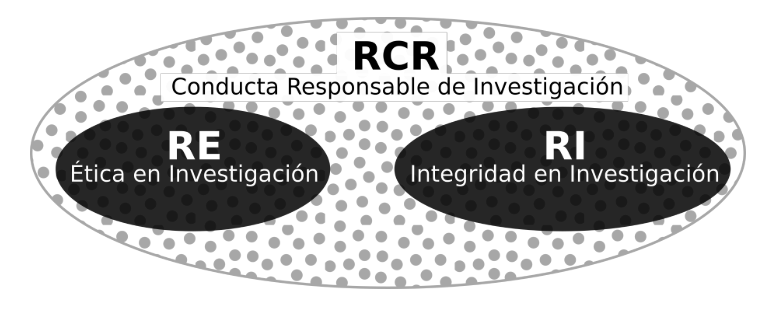
\includegraphics[width=1\linewidth]{docs/images/rcr}

\}

\textbackslash caption\{Conducta Responsable de Investigación. Imagen de \citet{abrilruiz_Manzanas_2019} basada en \citet{steneck_Fostering_2006}\}\label{fig:rcr}
\textbackslash end\{figure\}
Dentro de la RCR, la ética de investigación está relacionada al comportamiento académico visto desde la óptica de los principios morales \citep{steneck_Fostering_2006}, lo que se expresa en tópicos como el uso de datos, los consentimientos informados o el trato con pacientes -en el caso de las ciencias biomedicas-, por dar algunos ejemplos. La definición que ofrece \citet{steneck_Fostering_2006} señala que la ética de investigación se define como ``el estudio crítico de los problemas morales asociados o que surgen en el curso de la investigación'' (p.56) En cámbio, la integridad en investiación se entiende como ``poseer y adherirse firmemente a las normas profesionales, tal y como las señalan las organizaciones profesionales, las instituciones de investigación y, en su caso, el gobierno y el público'' \citep[p.56]{steneck_Fostering_2006}. A diferencia de la ética de investigación, el concepto de integridad está regido por los estándares profesionales más que por los principios morales, su función es plantear una guía clara para la conducta investigativa, de ahí que sea el concepto utilizado por distintos códigos de conducta \citep[ver][]{abrilruiz_Manzanas_2019}.

\textbackslash begin\{figure\}{[}H{]}

\{\centering 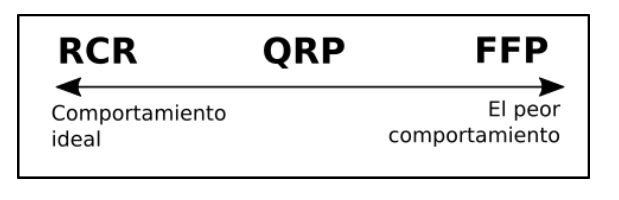
\includegraphics[width=1\linewidth]{docs/images/grad}

\}

\textbackslash caption\{Gradación del comportamiento integro en investigación. Imagen de \citet{abrilruiz_Manzanas_2019} basada en \citet{steneck_Fostering_2006}\}\label{fig:grad}
\textbackslash end\{figure\}
Habiéndonos situado dentro del concepto de integridad en la investigación, podemos pasar a delinear las principales prácticas que atentan contra él y que se han propuesto como factores que contribuyen a la crisis en la ciencia. Tanto \citet{steneck_Fostering_2006} como distintos códigos de conducta de universidades e instituciones de financiamiento \citep[ver][]{abrilruiz_Manzanas_2019} evalúan las prácticas de investigación en un continuo, que representa cuánto adhieren los investigadores a los principios de integridad cientifica. La Figura N° \ref{fig:grad} esquematiza esta idea mostrando dos extremos, donde a la izquierda está el mejor comportamiento (RCR), y a la derechaa el peor comportamiento (FFP). Las FPP son un abreviación en lengua inglésa para referirse a \emph{Fabrication, Falsification, Plagiarism} (Invención, Falsificación y Plagio), también conocidas como \emph{mala conducta académica}-. En el medio del continuo están las \emph{prácticas cuestionables de investigación} (QRP, por sus siglas en inglés) las cuáles refieren a ``acciones que violan los valores tradicionales de la empresa de investigación y que pueden ser perjudiciales para el proceso de investigación'' \citep[\emph{National Academies of Science} 1992 en][p.58]{steneck_Fostering_2006}. Las QRP se caracterizan porque tienen el potencial de dañar la ciencia, en tanto las FFP la dañan directamente.

Comprendidos ambos conceptos, veamos las situaciones que podrían categorizarse como FFP y las que podrían concebirse como QRP.

\hypertarget{mala-conducta-acaduxe9mica-ffp}{%
\subsection{Mala conducta académica (FFP)}\label{mala-conducta-acaduxe9mica-ffp}}

La mala conducta académica suelen ser situaciones polémicas y que muchas veces alcanzan gran conbertura mediatica. El libro de \citet{abrilruiz_Manzanas_2019} hace una revisión de una serie de situaciones, en distintas discplinas y años, en las que investigadores han sido descubiertos cometiendo prácticas que atentan directamente a la ciencia. Las situaciones son variadas, existen casos de manipulación de imagenes, exageración de lo registros de laboratorio, o de plano la invención de conjuntos de datos enteros. En esta sección veremos el caso de Diderik Stapel como ejemplo de malas prácticas de investigación y plantearemos la relación que tiene con la transparencia en la investigación.

\hypertarget{diderik-stapel}{%
\subsubsection{Diderik Stapel}\label{diderik-stapel}}

Probablemente, el caso de Diderik Stapel sea uno de los más emblématicos y representativos de este problema. Diderik Stapel era un investigador de la \emph{Tilburg University} que se dedicaba al campo de la psicología social. Su carrera se caracterizó por una trayectoria ejemplar, obtuvo su M.A en psicolgía y comunicaciones el año 1991, se doctoró en psicología social el año 1997 y trabajó como profesor asociado primero en la \emph{University of Gronigen} (2000-2006) y dede el 2006 en la Tilburg University. Fue fundador del \emph{Tilburg Institute for Behavioral Economics Research}, del cuál el 2010 se convirtió en decano. Así también, fue galardonado con el premio a la trayectoria académica por la \emph{Social of Experimental Social Psychology}. En breve, Stapel era una figura de alto estatus en el mundo académico, entre 1995 y 2015 publicó aproximadamente 150 artículos en revistas cientificas, algunas de las más prestigiosas (e.g.~\emph{Science}). Sin embargo, el año 2011 se confirmó que gran parte de su trayectoria académica era una farsa.

Después de la verificación de su culpa ante acusaciones de malas prácticas, la carrera de Diderik Stapel acabó. Fue desvinculado de la Tilburg University, se le rebocó su título de doctorado y toda su trayectoria académica fue investigada acusiociamente. El informe final de la investigación encontró que más de 50 de sus artículos eran fraudulentos. De hecho, Stapel ocupa el tercer lugar en con 58 artículos listados en \emph{Retraction Watch} (\url{https://retractionwatch.com/}), una plataforma que se dedica a sistematizar y mantener una lista actualizada sobre retracciones de artículos . A efectos de este escrito, lo que más destacable es que Stapel cometió conductas de mala conducta académica durante más de 15 años. La pregunta es ¿cómo fue esto posible? ¿cómo ninguno de sus colegas, alumnos o co-autores se dio cuenta de sus malas prácticas? La respuesta breve es por la falta de transparencia durante el proceso de investigación.

Los artículos periodisticos que han profundizado en el caso han relatado parte del proceso investigativo de Stapel \citep[e.g.][]{carey_Fraud_2011}. Dentro de los procesos de producción y análisis de datos, Stapel se caracterizaba por hacer todo el trabajo solo y ``a puertas cerradas''. Es decir, nadie más que él tenía acceso a los datos brutos, ni támpoco a la ejecución de las pruebas estadísticas. Generalmente, Stapel compartía con sus colegas y alumnos de doctorado la base de datos lista, con las pruebas estadísticas ya hechas y, claro está, con resultados estadísticamente significativos. Estas prácticas no causaron sospechas durante muchos años, es más, a muchos de sus estudiantes les parecía una práctica normal y eficiente. Además, con el estatus de Stapel ¿qué podría estar mal? Sin embargo, era a raíz de esta práctica que Stapel tenía la oportunidad de inventar y falsificar datos a su conveniencia. Esto explica en gran parte de su trayectoría académica llena de grandes hallazgos y una producción académica increible.

El caso de Stapel deja un punto importante sobre la mesa: la falta de transparencia en el proceso investigativo dio cabida a la mala conducta académica. Cómo nadie más colaboraba con el procesamiento de datos, ni támpoco parecía extraño que así fuera, las oportunidades para la falsificación de los datos estaba abierta. Ahora, esta no es necesariamente una relación de causalidad, la falta de transparencia no tiene porque terminar en conductas como fabricación o falsificación de datos. Sin embargo, tal y como lo argumentan \citet{oboyle_Chrysalis_2017} si son una oportunidad para violaciones a la integridad cientifíca más sutiles, tales como las QRP.

\hypertarget{pruxe1cticas-cuestionables-de-investigaciuxf3n-qrp}{%
\subsection{Prácticas cuestionables de investigación (QRP)}\label{pruxe1cticas-cuestionables-de-investigaciuxf3n-qrp}}

Recordemos, las QRP son prácticas que en si mismas no dañan directamente la empresa cientifica, pero si tienen el potencial de hacerlo. Son prácticas que alteran el correcto funcionamiento del método cientifico. En la literatura, existen una variedad de términos que se utilizan para describir las prácticas cuestionables, asi como también distintas listas de prácticas que han emitido instituciones . \citet{abrilruiz_Manzanas_2019} hace una recopilación y traducción de distintos códigos de conducta de distintas universidades y organismos, el cuál nosotros sistematizamos en la Tabla N° \ref{tab:tabqrp}. La tabla muestra un conjunto de prácticas divididos en cuatro categorías, de acuerdo a si las prácticas tienen que ver con: el diseño y el procesamiento de los datos, la redacción y el reporte de los resultados, temas de citación y uso de ideas ajenas y, por último, sobre relaciones con otros actores en el campo de la ciencia.

\begin{table}[!h]

\caption{\label{tab:tabqrp}Algunas situaciones de QRP}
\centering
\fontsize{10}{12}\selectfont
\begin{tabu} to \linewidth {>{\raggedright\arraybackslash}p{5 cm}>{\raggedright\arraybackslash}p{5 cm}}
\toprule
Dimensión & Práctica\\
\midrule
 & Ignorar ciertos aspectos de los requerimientos de las personas participantes.\\
\cmidrule{2-2}
 & Pasar por alto el uso de datos cuestionables o de interpretaciones cuestionables que otros hacen.\\
\cmidrule{2-2}
 & Cambiar partes de un estudio como respuesta a la presión de una fuente de financiación\\
\cmidrule{2-2}
 & Eliminar observaciones de los análisis basados en la intuición de que eran inexactos.\\
\cmidrule{2-2}
 & Redondear un valor p (por ejemplo, reportar que un p-value de 0,054 es menor a 0,05)\\
\cmidrule{2-2}
 & Eliminación, adición o alteración de datos después de pruebas de hipótesis.\\
\cmidrule{2-2}
 & Supresión selectiva o adición de variables.\\
\cmidrule{2-2}
\multirow{-8}{5 cm}{\raggedright\arraybackslash Diseño y procesamiento} & Invertir la dirección o reformular hipótesis para respaldar los datos\\
\cmidrule{1-2}
 & Ampliar de manera innecesaria la bibliografía de un estudio.\\
\cmidrule{2-2}
 & Tergiversar los logros de la investigación.\\
\cmidrule{2-2}
 & Exagerar la importancia y la relevancia práctica de los resultados.\\
\cmidrule{2-2}
 & Retener detalles de la metodología de investigación (e.g. no reportar todas las variables dependientes de un estudio)\\
\cmidrule{2-2}
 & Retener resultados de la investigación (e.g. no presentar datos que contradicen una propia investigación previa).\\
\cmidrule{2-2}
 & Establecer publicaciones o brindar apoyo a publicaciones que no cumplen el proceso de control de calidad de la investigación\\
\cmidrule{2-2}
 & Publicar los mismos datos o resultados en dos o más publicaciones.\\
\cmidrule{2-2}
 & Selectivamente reportar estudios que "funcionaron".\\
\cmidrule{2-2}
 & Reportar hallazgos inesperados como previstos desde el principio.\\
\cmidrule{2-2}
\multirow{-10}{5 cm}{\raggedright\arraybackslash Redacción, reporte y publicación} & Afirmar que los resultados no se ven afectados por variables demográficas cuando uno no está realmente seguro (o sabe que lo hacen).\\
\cmidrule{1-2}
 & Manipular la autoría o denigrar el papel de otros investigadores en las publicaciones.\\
\cmidrule{2-2}
 & Asignar inapropiadamente los crédios de autoría.\\
\cmidrule{2-2}
 & Volver a publicar partes sustanciales de publicaciones propias anteriores, incluidas las traducciones, sin citar debidamente el original ("autoplagio").\\
\cmidrule{2-2}
 & Citar de forma selectiva para mejorar los propios resultados o para complacer a los editores, los revisores o los colegas.\\
\cmidrule{2-2}
 & Usar ideas de otros sin obtener permiso o dar crédito\\
\cmidrule{2-2}
\multirow{-6}{5 cm}{\raggedright\arraybackslash Citación y autoría} & Uso no autorizado de información confidencial en relación con la propia investigación.\\
\cmidrule{1-2}
 & Permitir que los patrocinadores pongan en peligro la independencia en el proceso de investigación con el fin de introducir sesgos.\\
\cmidrule{2-2}
 & Acusar a un investigador de conducta indebida u otras infracciones de forma maliciosa.\\
\cmidrule{2-2}
 & Retrasar u obstaculizar inadecuadamente el trabajo de otros investigadores.\\
\cmidrule{2-2}
 & Emplear la experiencia profesional propia para alentar a que se incumpla la integridad de la investigación.\\
\cmidrule{2-2}
 & Ignorar supuestos incumplimientos de la integridad de la investigación cometidos por terceros o encubrir reacciones inadecuadas a conductas indebidas.\\
\cmidrule{2-2}
 & No divulgar adecuadamente la participación en empresas cuyos productos se basan en la investigación de uno.\\
\cmidrule{2-2}
\multirow{-7}{5 cm}{\raggedright\arraybackslash Relaciones con otros} & Relaciones con estudiantes, sujetos de investigación o clientes que pueden ser interpretadas como cuestionables.\\
\cmidrule{1-2}
 & \\
\bottomrule
\end{tabu}
\end{table}

Existen una serie de estudios que han intentado medir directamente la existencia de estas prácticas a través de encuestas. \citet{fanelli_How_2009} hizo un metanálisis que tenía por objetivo sistematizar los resultados de estudios que hasta esa fecha habían abordado las prácticas de investigación desde encuestas cuantitativas. Los resultados mostraron que un 1.97\% de investigadores había inventado datos al menos una vez (FFP) y que un 33.7\% había realizado alguna vez una QRP como ``borrar puntos de los datos basados en un sentimiento visceral''. Un estudio más reciente, también basado en encuestas cuantitativas sobre prácticas, es el de \citet{john_Measuring_2012}. En este estudio, los resultados mostraron que un 36.6\% de quienes participaron alguna vez habían práctiado alguna QRP. En detalle, analizando los porcentajes práctica a práctica se halló que el 50\% de los psicologos encuestados alguna vez reportaron selectivamente estudios que apoyaran su hipótesis; un 35\% alguna vez reportaron resultados inesperados como esperados; y un 2\% alguna vez reportó datos falsos. Estos estudios son una primera aproximación a la existencia de las QRP en la ciencia.

Existen ciertas prácticas que han sido tratadas con más enfásis en la literatura, y que son las que queremos destacar acá. Por un lado, está el \emph{sesgo de publicación}, el cual significa, a grandes rasgos, que un artículo es públicado en base a sus resultados. Especificamente, el sesgo de publicación ocurre cuando el criterio determinante para que un artículo sea públicado es que sus resultados sean signiificativos, en desmedro de la publicación de resultados no signifcativos. El estudio de \citet{franco_Publication_2014} logra cuantificar esta situación bastante bien y esclarecer el \emph{file drawer problem} (en español: problema del cajón de archivos), que hace alusión a los resultados perdidos dentro de un cuerpo de evidencia \citep[p.39]{christensen_Transparent_2019}. \citet{franco_Publication_2014} encontraron que, efectivamente, los resultados nulos tienen un 40\% menos de probabilidades de ser públicados en revistas cientificas, en comparación a estudios con resultados significativos. Es más, muchas veces los resultados nulos nisiquiera llegan a ser escritos: más de un 60\% de los experimentos que componen la muestra del estudio de \citet{franco_Publication_2014} nunca llegaron a ser escritos, en contraste al menos del 10\% de resultados significativos.

El principal problema del sesgo de publicación es que puede impactar en la credibilidad de cuerpos enteros de literatura. Existen ejemplos de cuerpos de literatura que se han hallado sesgados, como el \emph{Value of Statistical Life} (Valor de la Vida Estadística) y el de salario mínimo y desempleo, ambos en economía \citep[para detalle ver p.42 y p.46 en][]{christensen_Transparent_2019}. También, a partir del desarrollo de distintos métodos de detección, se ha podido diagnosticar el sesgo de publicación en importantes revistas en economía \citet{brodeur_Star_2016}, sociología y ciencias políticas \citep{gerber_Publication_2008, gerber_Statistical_2008}.

Otra práctica bastante cuestionada es el \emph{p-hacking}, que de forma literal sería un ``hackeo'' de los valores p.~El \emph{p-hacking} se da cuando el procesamiento de los datos tiene por objetivo obtener resultados significativos. Si el sesgo de publicación afecta la credibilidad de un cuerpo de literatura, el \emph{p-hacking} afecta a la credibilidad de los artículos mismos, ya que al forzar la signifcancia estadística la probabilidad de que en realidad estemos frente a un falso positivo aumenta. Un trabajo que da sustento a esta idea es el de \citet{simmons_FalsePositive_2011}, quienes calculan la posibilidad de obtener un falso positivo (error Tipo I) de acuerdo a al nivel de manipulación intencionada de los datos. El resultado principal es que a medida que aumenta la cantidad de manipulación en los datos, la posibilidad de obtener un falso positivo aumenta progresivamente.

El \emph{p-hacking} también contribuye a sesgar cuerpos enteros de literatura. Para diagnosticar esto se ha utilizado una herramienta denominada \emph{p-curve}, la cual ``describe la densidad de los \emph{p-values} reportados en una literatura, aprovechando el hecho de que si la hipótesis nula no se rechaza (es decir, sin efecto), los p-values deben distribuirse uniformemente entre 0 y 1'' \citep[p.67.]{christensen_Transparent_2019}. De esta manera, en cuerpos de literatura que no sufran de p-hacking, la distribución de p-values debería estar cargada a la izquierda (siendo precisos, asimetrica a la derecha), en cambio, si existe sesgo por p-hacking la distribución de p-values estaría cargada a la derecha (asimetría a la izquierda). \citet{simonsohn_Pcurve_2014} proponen esta herramienta y la prueban en dos muestras de artículos de la \emph{Journal of Personality and Social Psychology (JPSP)}. Las pruebas estadísitcas consistieron en confirmar que la primera muestra de artículos (que presentaban signos de p-hacking) estaba sesgada, en cambio la segunda muestra (sin indicios de p-hacking), no lo estaba. Los resultados corroboraron las hipótesis, en detalle, los artículos que presentaban solamente resultados con covariables, resultaron tener una p-curve cargada a la derecha (asimetrica a la izquierda).

Por último, pero no menos importante existe la práctica del \emph{HARKing}. El nombre es una nomenclatura en lengua inglesa: \emph{Hypothesizing After the Results are Known}, que literalmente significa establecer las hipótesis del estudio una vez que se conocen los resultados. El principal problema de esta práctica es que confunde los dos tipos de razonamiento que están a la base de la ciencia: el exploratorio y el confirmatorio. El objetivo principal del razonamiento exploratorio es plantear hipótesis a partir de un análisis de datos. En cambio, el razonamiento confirmatorio busca plantear hipótesis basado en teoría y contrastar esas hipótesis con datos empíricos. Como señala \citet{nosek_preregistration_2018}, cuando se confunden ambos tipos de análisis y se hace pasar un razonamiento explortorio como confirmatorio se está cometiendo un sesgo inherente, ya que se está generando un razonamiento circular: se plantean hipótesis a partir del comportamiento de los datos y se confirman las hipótesis con esos mismos datos.

\hypertarget{que-podemos-hacer}{%
\section{¿Que podemos hacer?}\label{que-podemos-hacer}}

Tanto en las ciencias sociales, como en otras disciplinas han ido emergiendo una variedad de recomendaciones que contribuyen a la adopción de la transparencia. Por ejemplo, \citet{cruwell_Easy_2018} propone formar investigadores y estudiantes a partir de la promoción de siete principales tópicos: entender la ciencia abierta; acceso abierto; la importancia de los datos, material y código abierto, los análisis reproducibles; los pre-registros; la replicación y, por último, la enseñanza de la ciencia abierta. Cada uno de estos tópicos son un paso para lograr avanzar hacia una ciencia más abierta y transparente. De forma similar, \citet{miguel_Promoting_2014} enfatiza en tres ideas: el \emph{disclosure} (divulgación), los pre-registros y los datos y materiales abiertos. La divulgación consta de que los investigadores deben declarar todo tipo de procesamiento realizada a los datos y detallar como se llégó a las muestras finales. Los preregistros son una forma de ser más transparente con los procedimientos y dividir los tipos de formulación de hipótesis. Los datos y materiales abiertos permite que otros investigadores puedan reproducir el trabajo, hacer otras pruebas de hipótesis, identificar malas prácticas etc. También \citet{lindsay_Seven_2020} discute los efectos que tienen el sesgo de publicación y otras prácticas similares en la credibilidad de la ciencia, proponiendo siete pasos para mejorar la transparencia: decir la verdad, por ejemplo, si la idea de investigación surgió analizando datos plantearlo de esa manera; evaluar la comprensión de la estadística inferencial; estandarizar la aproximación para probar las hipótesis, por ejemplo, realizar un plan de análisis; hacer un manual de laboratorio (en el caso de diseños experimentales); hacer abiertos los materiales, datos y análisis; abordar las limitaciones de la generabilidad de las conclusiones; y por último, considerar enfoques colaborativos para conducir investigaciones. \citet{oboyle_Chrysalis_2017} proponen tres simples consejos para hacer la ciencia más transparente: incluir una clausulas éticas en el envío de manuscritos que declaren no haber cometido QRP, qué todo artículo original (e.g.~tesis doctoral) debe estar disponible para descarga y que las revistas cuenten con un espacio dedicado a replicación.

Una propuesta sistemática para adoptar la transparencia, que incluye varias de las recomendaciones mencionadas son las \emph{Transparency and Openess Promotion (TOP) Guidelines} (Guías para la Promoción de la Transparencia y la Accesibilidad). Estos son principios que buscan alcanzar un formato de investigación reproducible a través del aumento de la transparencia en el proceso y los productos de investigación \citep{nosek_Transparency_2014}. Estos principios sirven de guía tanto para la adopción de buenas prácticas en los investigadores, como para que las revistas académicas puedan adherir progresivamente al ideal de transparencia en la ciencia. Son ocho principios:

\begin{enumerate}
\def\labelenumi{\arabic{enumi}.}
\tightlist
\item
  Citación
\item
  Transparencia de datos
\item
  Transparencia de métodos análiticos (código)
\item
  Transparencia de los materiales
\item
  Transparencia del diseño y el análisis
\item
  Preregistro de estudios
\item
  Pre registro de planes de análisis
\item
  Replicación
\end{enumerate}

A grandes rasgos, el principio de citación propone que las normas de citado deben ampliarse también a los datos y códigos, permitiendo reconocer su autoría intelectual \citep{nosek_Promoting_2015}. Los principios de transparencia de datos, métodos análiticos, materiales y diseño y análisis (2 a 5) refieren a la transparencia en su forma más concreta: la apertura del proceso de investigación para su evaluación. El detalle puesto a los principios responde a la generelabizilidad que se le busca dar a los principios. Por ejemplo, un estudio observacional cuantitativo no tiene material que transparentar, pero si datos y métodos análiticos. Asi también, un estudio cualitativo quizás no tenga código que transparentar, pero si un diseño y una bitacora detalla del proceso de análisis. En el caso de los principios relacionados al pre-registro, \citet{nosek_Promoting_2015} argumenta que registrar los estudios los hace más descubribles, incluso si no son públicados. Asi también, los preregistros del plan de análisis contribuyen a distinguir entre los análisis confirmatorios y explotatorios (ver \citet{nosek_preregistration_2018} para un manejo detalado del tema). Por último, el principios de replicación fomenta las oportunidades para la corrección de artículos y redirecciona la investigación en vías más prometedoras \citep{nosek_Promoting_2015}.

Cada uno de estos principios cuenta con tres niveles, que sirven para medir el grado de inclusión de la transparencia por parte de una revista cientifica (ver Figura N° \ref{fig:tabtop} para detalle). La adopción de prácticas transparentes va desde el nivel 1, siendo lo menos transparente, hasta el nivel 3 siendo lo más transparente. Se añade un nivel 0 que no cumple los estandares de transparencia con la finalidad de tener una comparación. Por ejemplo, para los estandares de transparencia del método de análisis (código), el nivel 1 dicta que las revistas deben solicitar la existencia del código de análisis, en cambio, el nivel 3 es más estricto en plantear que el código de análisis debe estar almacenado en un repositorio confiable y que el análisis será reproducido durante el proceso de revisión. El mismo método se puede aplicar para la el preregistro del plan de análisis. En el nivel 1 las revistas promueven el uso de preregistros, en cambio, en el nivel 3 los preregistros son obligatorios y también reconocidos. En suma, las TOP Guideliness son una iniciativa que contribuye a la apertura en la ciencia proponiendo nuevas prácticas para los requerimientos de las revistas.

\begin{figure}[H]

{\centering 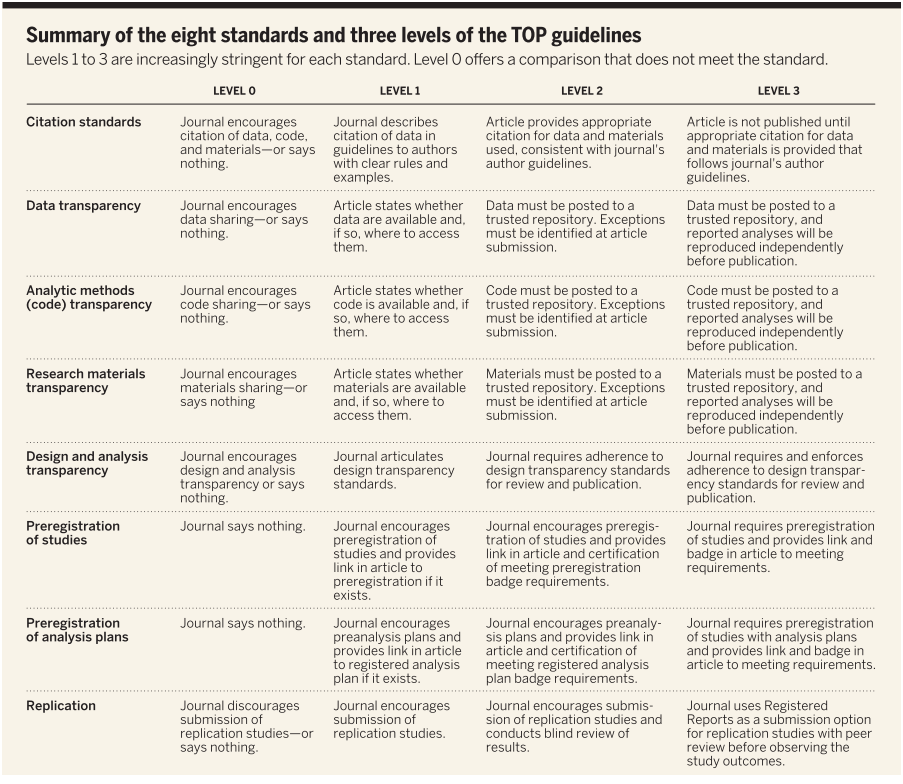
\includegraphics[width=1\linewidth]{docs/images/table_top} 

}

\caption{Variaciones por dimensión de transparencia}\label{fig:tabtop}
\end{figure}

Como podemos ver, en general las recomendaciones sobre transparencia giran en torno a los preregistros, los datos y materiales abiertos y la replicación. En la siguiente sección profundizaremos en los preregistros como una forma de aumentar la transparencia durante el proceso de investigación.

\hypertarget{reproducibilidad}{%
\chapter{Reproducibilidad}\label{reproducibilidad}}

¿Cuántas veces nos hemos enfrentado a un trabajo publicado que no comparte sus materiales, y que por tanto, es imposible acceder a los procedimientos que dieron luces de sus resultados? En el marco de la denominada ``crisis de la ciencia'', la comunidad científica se ha organizado para dar salida a este problema a través de una diversidad de iniciativas que, a modo general, buscan promover los principios de la ciencia abierta. En este sentido, dichas iniciativas han puesto sus esfuerzos en contribuir con herramientas que permitan dar salida a los problemas en torno a la transparencia de los procesos de investigación y la \textbf{reproducibilidad} en la investigación empírica. En este apartado, revisaremos cómo ha sido entendido este problema y luego se presentarán las propuestas de tres iniciativas en torno a cómo abordar la reproducibilidad en las ciencias sociales empíricas.

\hypertarget{cuxf3mo-se-entiende}{%
\section{Cómo se entiende}\label{cuxf3mo-se-entiende}}

En la discusión sobre los problemas de transparencia en torno a los procesos y procedimientos de investigación, se vuelve necesario precisar de qué manera es entendido el concepto de reproducibilidad en la ciencia. En esta línea, la laxitud en que ha se ha empleado el término ha llevado a definiciones poco claras, lo cual ha generado una tendencia a confundir lo que refiere a la transparencia de un proceso único que ya ha sido realizado, con un proceso nuevo y que puede realizarse de manera reiterativa, obteniendo los mismos resultados.

La discusión en torno a cómo se entiende la \textbf{reproducibilidad}, habitualmente lleva al contraste respecto al concepto de \textbf{replicabilidad}. Al respecto \citet{earth_Reproducibility_2019} menciona que con el incremento de las herramientas computacionales a principios de los años 90', el término de ``investigación reproducible'' era concebido como las investigaciones que proveían un compendio detallado de la documentación, código y datos que permitieran obtener los mismos resultados publicados por los autores, enfatizando que los análisis fueran transparentes y claros con el objetivo de ser verificados por sus pares. Por otro lado, los autores sostienen que en otras disciplinas, el concepto de reproducibilidad era asociado a investigaciones independientes entre sí en términos de los datos empleados, los materiales e implementación, lo cual estaría orientado a robustecer o cuestionar la evidencia previa \citep[pp 33-34]{earth_Reproducibility_2019}. Actualmente, a esta práctica se la entiende como ``replicabilidad'' de una investigación y no debe ser confundida con el concepto de ``reproducibilidad'' \citep{barba_Terminologies_2018}.

\citet{barba_Terminologies_2018} sugiere que la confusión entre reproducibilidad y replicabilidad ha contribuido a obstaculizar las prácticas en ambas dimensiones. En una revisión reciente realizada por la autora se han identificado al menos tres escenarios o versiones de cómo se entienden ambos conceptos en una amplia gama de disciplinas que van desde las ciencias sociales hasta estudios clínicos. El primer escenario (A), y a la vez el más común, es donde el uso de ambos conceptos es indistinto, contribuyendo a la ya mencionada confusión. El segundo escenario (B1) es cuando la reproducibilidad es entendida como la situación que los datos originales y el código de análisis son empleados para \textbf{regenerar} los resultados originales, mientras que la replicabilidad es entendida cuando investigadores o equipos independientes utilizan datos nuevos para obtener los mismos resultados que la investigación previa. Finalmente, un tercer escenario (B2) es cuando la reproducibilidad es entendida cuando investigadores o equipos independientes obtienen los mismos resultados empleando sus propios datos y métodos, mientras que la replicabilidad es entendida cuando investigadores o equipos independientes llegan a los mismos resultados empleando los ``artefactos digitales'' \footnote{\citet{barba_Terminologies_2018} lo define como un compendio que detallar la estrategia de medición, diseño del estudio o código de análisis originales de un autor} originales del autor con menores o mayores modificaciones, los cuales han sido puestos previamente a disposición de sus pares. La Figura \ref{fig:scenarios} ilustra cómo podemos entender los escenarios B1 y B2 en relación a la distinción entre reproducibilidad y replicabilidad.

\begin{figure}[H]

{\centering 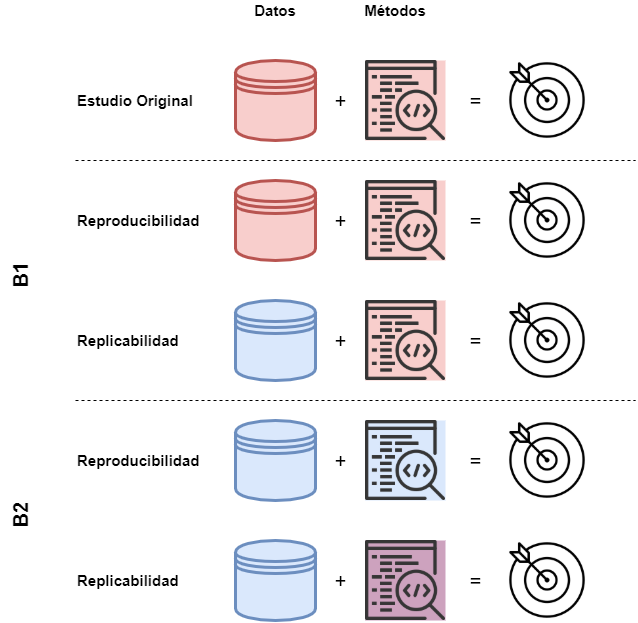
\includegraphics[width=0.75\linewidth]{docs/images/reproducibility} 

}

\caption{Escenarios B1 y B2 en reproducibilidad y replicabilidad.}\label{fig:scenarios}
\end{figure}

En las ciencias sociales, el debate en torno a la investigación reproducible y la replicabilidad no ha estado ausente. Como fue reseñado en la sección anterior, existen casos icónicos en torno a prácticas cuestionables de investigación que han afectado la confianza en la investigación científica, lo cual ha contribuido a incrementar los esfuerzos por una ciencia social abierta y reproducible \citep{breznau_Does_2021, nosek_Promoting_2015}. En los tres escenarios descritos por \citet{barba_Terminologies_2018}, las ciencias sociales han experimentado de manera diversa el ajuste hacia una cultura de mayor apertura y precisión en torno a los problemas de la crisis de reproducibilidad, principalmente a través del estudio sistemático de dicha problemática, dentro de lo cual la psicología ha sido un pionera en proveer evidencia para este debate \citep{opensciencecollaboration_Estimating_2015, gilbert_Comment_2016}. Al respecto \citet{bishop_Rein_2019} sostiene que una de las principales amenazas para el progreso de la ciencia en general ha sido a la falta de reproducibilidad de los resultados (\emph{irreproducibility}), lo cual ha afectado principalmente la robustez y credibilidad de la evidencia reportada por las investigaciones, problema que también ha sido identificado en las ciencias sociales, principalmente por la falta de precisión en los procedimientos y las barreras de acceso a materiales clave del proceso de análisis \citep{freese_Replication_2017}.

Entonces, retomando la distinción clave entre lo que entendemos por \textbf{reproducibilidad} y \textbf{replicabilidad}, en su revisión, \citet{barba_Terminologies_2018} sugiere que una manera de entender y distinguir ambos conceptos de manera minimalista puede descansar en el carácter de los \emph{datos} y los \emph{métodos}. Al respecto \citet{nosek_Promoting_2015} sostiene que en lo que refiere a estas dos dimensiones, los niveles en que una publicación los incorpora es gradual y puede entenderse como un continuo o espectro \citep{peng_Reproducible_2011}, y por tanto, el nivel en que se cumplen con determinados criterios nos permite definir el carácter de una investigación en términos de su reproducibilidad. Por ejemplo, la Figura \ref{fig:espectro} nos muestra cómo podemos caracterizar una investigación publicada en torno al acceso y vinculación entre código y datos. Por un lado, se observa que en el polo donde únicamente disponemos de la publicación, se entiende como la ausencia de reproducibilidad. Por otro lado, en la medida que incrementa el acceso a los materiales, y se explicita el enlace entre ellos, se puede caracterizar a una publicación como reproducible. \footnote{En la figura original, \citet{peng_Reproducible_2011} muestra el polo derecho como el mejor escenario y lo clasifica como \emph{Full replication}, sugiriendo que el mejor estándar para poner a prueba los hallazgos de una investigación científica es la replicación, pero en la ausencia de dicha posibilidad la reproducibilidad de los resultados debiese ser un estándar mínimo}

\textbackslash begin\{figure\}{[}H{]}

\{\centering 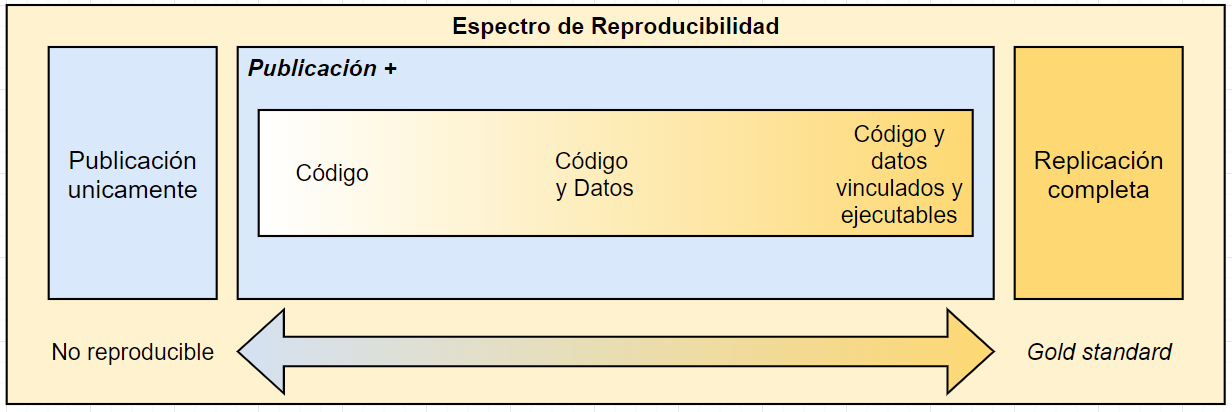
\includegraphics[width=0.75\linewidth]{docs/images/repro-spectrum}

\}

\textbackslash caption\{Espectro de Reproducibilidad. Traducción propia en base a \citet{peng_Reproducible_2011} \}\label{fig:espectro}
\textbackslash end\{figure\}

Como sugiere \citet{nosek_Promoting_2015}, el problema de la ausencia o falta de reproducibilidad debe ser abordado a través de un cambio en las prácticas de investigación, para lo cual se requiere, por un lado, de una disposición por parte de la comunidad científica, es decir a que se le atribuya un \emph{sentido} positivo a estas prácticas. Sin embargo, \citet{peng_Reproducible_2011} sostiene que una de las principales barreras para promover estas prácticas ha sido la falta de mecanismos que faciliten la distribución de la investigación reproducible, como también la poca claridad respecto de los estándares asociados a ello.

\hypertarget{iniciativas}{%
\section{Iniciativas}\label{iniciativas}}

\hypertarget{berkeley-initiative-for-transparency-in-the-social-sciences}{%
\section{Berkeley Initiative for Transparency in the Social Sciences}\label{berkeley-initiative-for-transparency-in-the-social-sciences}}

\hypertarget{objetivos-y-visiuxf3n}{%
\subsection{Objetivos y visión}\label{objetivos-y-visiuxf3n}}

Esta iniciativa busca promover la credibilidad en la evidencia generada por las ciencias sociales a través de mecanismos de avanzada para la transparencia, reproducibilidad y prácticas éticas en la investigación social empírica. Desde esta premisa, ha desarrollado y puesto a disposición de la comunidad científica una serie de herramientas en colaboración con estudiantes, investigadores, entidades académicas y fundaciones de la sociedad civil al alero de tres principios orientadores.

Generar evidencia en torno a problemas y soluciones a través de los investigadores y la comunidad de BITSS quienes han liderado investigaciones meta-analíticas con atención en las ciencias sociales.
Incrementar el acceso a la enseñanza de la ciencia abierta, a través del fortalecimiento de prácticas para reconocer y conducir investigación social transparente y reproducible a través del entrenamiento de investigadores jóvenes, acceso a materiales, apoyo financiero y la consolidación de una red de colaboración.\\
Fortalecer el ecosistema científico, estableciendo condiciones para investigadores e instituciones para contribuir a un cambio efectivo y equitativo en las normas que permitan una consolidación de una política interna orientada a la ciencia abierta y al desarrollo de protocolos en esta dirección.

Como se ha señalado, esta iniciativa se orienta bajo estos tres ámbitos o principios. Desde sus inicios, se han desarrollado una serie de componentes que buscan promover y dar soluciones a los problemas de transparencia y reproducibilidad en las ciencias sociales. En particular, nos interesa destacar algunas de las contribuciones en este ámbito que serán presentadas a continuación las cuales se pueden resumir en Evidencia, Educación y Recursos.

\hypertarget{contribuciuxf3n}{%
\subsection{Contribución}\label{contribuciuxf3n}}

En el ámbito de Evidencia, desde BITSS se ha realizado un esfuerzo por producir y sistematizar evidencia centralizadamente. En este contexto existe la \href{https://www.bitss.org/research-library/}{Research Library}, una base de datos de publicaciones científicas que engloba una serie de investigaciones meta-analíticas en el ámbito de las ciencias sociales, contribuyendo con un cuerpo de evidencia sistemática en torno a los problemas y soluciones sobre transparencia y reproducibilidad en las ciencias sociales sin precedentes. En este apartado, tanto los colaboradores como investigadores de BITSS ponen a disposición de la comunidad científica las investigaciones que han sido financiadas a través de las Social Science Meta-Analysis and Research Transparency (\href{https://www.bitss.org/ssmart-grants/}{SSMART}) grants, las cuales constituyen fondos orientados a contribuir a la investigación empírica en torno a la transparencia y reproducibilidad en disciplinas como la economía, ciencia política, psicología y ciencias sociales afines.

\hypertarget{herramientas-para-la-transparencia-y-irreproducibilidad}{%
\chapter{Herramientas para la transparencia y irreproducibilidad}\label{herramientas-para-la-transparencia-y-irreproducibilidad}}

En la sección anterior hemos hecho un repaso sobre la narrativa

\hypertarget{preregistros}{%
\section{Preregistros}\label{preregistros}}

\hypertarget{algunas-cosas-sobre-los-preregistros}{%
\subsection{Algunas cosas sobre los preregistros}\label{algunas-cosas-sobre-los-preregistros}}

Los preregistros son una marca temporal sobre las decisiones del diseño, el método y el análisis de un artículo cientifico y se suelen hacer antes del levantamiento de datos \citep{stewart_Preregistration_2020}. Básicamente, preregistrar un artículo o un proyecto implica que un grupo de investigadores dejarán por escrito una pauta de investigación a la cuál se atendrán lo más posible cuando desarrollen la investigación, especialmente la recopilación y el análisis de los datos. Ahora ¿por qué habría de hacer algo así? Llevar a cabo una investigación ya es lo suficientemente complejo como para añadirle una tarea adicional. La respuesta es que, cómo señalamos en secciones anteriores, los preregistros son una herramienta que permite hacerle frente a las QRP y, a la larga, contribuir a la realización de una ciencia de mayor calidad.

Ciertamente, los preregistros no son la respuesta a cada una de las QRP existentes, pero si son una herramienta eficaz para evitar las más frecuentes. En secciones anteriores hablamos de los sesgos de publiación, el p-hacking y el HARKing pues, cada uno de ellos puede ser evitado a partir de un preregistro. Primero, vimos que el sesgo de publicación se trataba de publicar selectivamente los resultados de inevstigación: resultados que no hayan sido significativos, o hipotésis que ``no funcionaron'' simplemente se omiten. Sin embargo, cuando existe un documento como un preregistro, el cual deja estipulado claramente las hipótesis que deben ponerse a prueba y los análisis que se emplearan para ello, se torna más dificil reportar selectivamente los resultados. Dicho de otra forma, cuando existe una pauta a la cual apegarse, la discrecionalidad en el reporte de los resultados disminuye. En el caso del p-hacking, el efecto del preregistro es parecido. Cómo vimos, el p hacking consistía en abusar de las pruebas estadísticas para obtener resultados significativos. ``Abusar'' en el sentido de buscar toda via posible para obtener un valor p que confirme las hipótesis planteadas. El hecho de preregistrar el plan de análisis y el procesamiento que se le efectuara a las variables permite evitar este tipo de búsqueda intencionada: como hay una guía que seguir, cualquier desviación debe ser justificada. En esta misma línea, un preregistro evita el HARKing ya que las hipótesis están previamente planteadas y no es posible cambiarlas una vez que se han visto los resultados. En suma, el plantear un registro \emph{a priori} de la investigación, disminuye la flexibilidad que suele dar paso a las QRP.

Si bien los preregistros pueden ser una herramienta en contra de las QRP, existen resquemores de los que es preciso hacerse cargo. Una de las principales preocupaciones es que el uso de preregistros tendería a coartar la creatividad y la producción de conocimiento exploratoria \citep{moore_Preregister_2016}. La lógica es que, como cada parte de la investigación debe ser registrada detalladamente previo a la recopilación, no queda espacio para la espontaneidad durante el análisis el análisis de datos. Nada puede estar más lejos del sentido de un preregistro. Más que inhibir la investigación exploratoria, el objetivo de expecificar una pauta a priori es poder separar lo que es la inevstigación confirmatoria (pruebas de hipótesis) y la exploratoria (generación de hipótesis) \citep{nosek_preregistration_2018}. En ese sentido, es posible la investigación exploratoria bajo el modelo de preregistros, solo que hay que especificarla como tal. Una segunda creencia es que realizar un preregistro añade un nivel de escrutinio mayor del necesario, es decir, como se conoce cada detalle, la investigación se vuelve un blanco fácil de críticas. Sin embargo, la situación es todo lo contrario \citep{moore_Preregister_2016}, por ejemplo, haber preregistrado un plan de análisis para una regresión logística binaria con datos que originalmente eran ordinales hará más creíble los resultados, ya que quienes evalúen la investigación tendrán pruebas de que el nivel de medición no se cambió solo para obtener resultados significativos. Una tercera idea en torno a los preregistros es que conllevan una gran inversión de tiempo y energía. Si bien es cierto que se añade un paso más al proceso de investigación, el avance en la temática ha logrado que existan una variedad de plantillas que hacen el proceso más rápido y eficiente. Desde una lógica racional, el tiempo que toma este paso nuevo en la investigación es un costo bajo en contraste a los beneficios que trae.

Una característica principal de los preregistros es que deben ser efectuados previo a la recoleccion de datos. Este requisito es lo que permite asegurar la credibilidad de los resultados, ya que, si no hay datos que alterar, entonces las probabilidades de que ocurra una QRP son básicamente nulas. Generalmente, para las ciencias médicas o la psicología experimental (discplinas donde cada vez se usan más los preregistros), esto no suele ser un problema ya que se utilizan diseños experimentales. Los diseños experimentales se apegan al método cientifico clásico: se plantean hipótesis basadas en la teoría, se diseña un experimento para probar esas hipótesis y luego se recopilan y analizan los datos para ver si dan soporte a las hipótesis planteadas. Sin embargo, ¿qué ocurre cuando trabajamos con datos pre-existentes? En muchas discplinas de las ciencias sociales los diseños experimentales son una pequeña fracción del conjunto de la literatura \citep[e.g.~según][ en 2010, un 3\% de los papers en las mejores revistas de economía eran experimentales]{card_Role_2011}, donde lo que prima son los diseños observacionales, los que suelen trabajar con datos administrativos o generados a partir de censos o encuestas. A diferencia de los estudios experimentales, los cuales deben generar de primera fuente el experimento que les permita testear sus hipótesis, en los estudios observacionales se utilizan datos ya existentes, lo cual afecta al principal componente de credibilidad de los preregistros: nada puede asegurar que los datos fueron analizados antes de la escritura del preregistro y que, por ejemplo, las hipótesis se estan planteando una vez conocidos los patrones significativos (HARKing). De ahi que nace la pregunta sobre la posibldad (y los útilidad) de utilizar preregistros en estudios con datos pre-existentes.

En la literatura sobre preregistros se han discutido los desafíos que implica preregistrar estudios que utilicen datos pre-existentes \citep[e.g.][]{editors_Observational_2014}. Existen posturas que proponen que, en realidad, no existe una forma creíble para preregistrar este tipo de estudios \citep{christensen_Transparency_2018}. No obstante, otras posturas han profundizado en las situaciones en las que aun es posible pre-registrar estudios con datos elaborados previamente. \citet{burlig_Improving_2018} propone tres escenarios donde el preregistro de datos observacionales es valioso. El primero es, básicamente, cuando los investigadores que diseñaron la investigación generan sus propios datos. En este caso, los investigadores sí pueden elaborar un preregistro previo a la recolección de datos. El segundo escenario se da cuando se preregistra un estudio que tenga como objeto de interés un suceso que aun no ha ocurrido, lo que se conoce como estudios prospectivos. Por ejemplo, un grupo de investigadores puede estar interesado en el efecto que tendrá la introducción de una ley en las prácticas sociales, o el efecto de un tratado en las variaciones del PIB. Para esos casos, el preregistro aun mantiene su validez original ya que, si bien los datos ya existen, no es posible hacer los análisis antes del preregistro porque el evento de interés no ha ocurrido. El tercer escenario ocurre cuando los datos existen, pero no están abiertos al público. En estos casos, es la accesibilidad lo que determina la credibilidad del preregistro. Por ejemplo, el grupo de investigadores que elaboraron los datos pueden establecer que serán accesibles con previo contacto y que se solicitará un preregistro. Por ende, en orden de analizar los datos, los investigadores interesados deberán elaborar un preregistro para utilizar los datos. Según \citet{mertens_Preregistration_2019}, también se pueden adoptar ciertas prácticas para asegurar la credibilidad de un preregistro con datos secundarios. Dos de ellas son: que el grupo de investigadores que analiza los datos sea distinto e independiente de quien propuso el diseño de investigación y que el equipo realice sintaxis de análisis con datos simulados, con tal de demostrar que las hipotésis ya existían previo a acceder a los datos. En suma, lo que permite mantener el efecto ``puro'' de un preregistro, es que los datos no hayan sido observados por ningún integrante del grupo de investigación que los analizará \citep{nosek_preregistration_2018}.

El principio básico de un preregistro entonces, es que los datos no deben haber sido observados previos al análisis. Sin embargo, según \citet{nosek_preregistration_2018} aun pueden existir ciertos sesgos en el planteamiento de hipótesis a raíz de cosas como el reporte de resultados descriptivos de la base de datos o las recomendaciones sobre cómo aproximarse a la base de datos. Este tipo de influencias son un poco más sútiles y es difícil deshacerse completamente de ellas. Es por esto que, quizás la recomendación más transversal y a la vez simple para pregistristrar análisis con datos secundarios, es ser sincero y detallado respecto a lo que se ha hecho y lo que no {[} \href{mailto:v@nosek_preregistration_2018}{\nolinkurl{v@nosek\_preregistration\_2018}}{]}. Si es que se ha leído el reporte descriptivo sobre la base de datos, estipularlo como tal. Es preciso transparentar cualquier tipo de aproximación a los datos previo haberlos analizados. Para lograr este nivel de detalle y ser eficiente con los tiempos y la comunicación hacia otros investigadores, es que existen plantillas predeterminadas para preregistrar distintos tipos de artículos. A continuación veremos las más comunes y nos centraremos en describir una de las más usadas y su variante para estudios que usen datos secundarios.

\hypertarget{manos-a-la-obra-cuxf3mo-utilizar-un-preregistro}{%
\subsection{Manos a la obra: cómo utilizar un preregistro}\label{manos-a-la-obra-cuxf3mo-utilizar-un-preregistro}}

En la práctica, preregistrar un artículo es básicamente sintetizar la información importante sobre nuestra investigación en una planitlla estandarizada, y alojar ese documento en un lugar público. Es por eso que el primer paso para elaborar un preregistro es elegir la plantilla correcta. Existen plantillas estandarizadas, que están estructuradas de tal forma que son útiles para preregistrar estudios de cualquier discplina, asi como también existen plantillas dedicadas a una disciplina o un conjunto de ellas. En la Tabla N° \ref{tab:tabprereg} se pueden ver algunas de las plantillas más usadas. Primero está el conjunto de plantillas que ofrece el Open Science Framework (OSF) dependiendo de las caracteristicas específicas del estudio. Luego, encontramos a la plantilla de AsPredicted que se caracteriza por su simpleza: son solo nueve preguntas que buscan recopilar la información sustancial para el preregistro de un artículo. También, están las plantillas de PROSPERO, ISRCTN y Bio-Protocol que se utilizan más en el campo de las ciencias biológicas o médicas. PROSPERO se focaliza en artículos de tipo review que tengan relación con la medicina, en tanto IRCTN busca ser una primera instancia de registro para ensayos clínicos. Bio-Protocol por su parte busca dejar el registro de protocolos detallados en la investigación biológica, con tal de complementar la sección de Método en los artículos. Las plantillas de AEA RCT, RIDIE y EGAP están más relacionadas a las ciencias sociales y áreas afines. la AEA RCT se focaliza en diseños experimentales para ciencias sociales, en tanto RIDIE es una herramienta para evaluaciones de impácto. EGAP busca ser una plantilla específica para temas de gobernanza y política. Como podemos ver, todas las plantillas tienen su campo de aplicación, sin embargo, aquí nos centraremos en las dos más unievrsales y conocidas: la de OSF y la de AsPredicted.

\begin{table}[!h]

\caption{\label{tab:tabprereg}Plantillas de preregistro}
\centering
\fontsize{10}{12}\selectfont
\begin{tabu} to \linewidth {>{\raggedright\arraybackslash}p{5 cm}>{\raggedright\arraybackslash}p{5 cm}>{\raggedright}X}
\toprule
Plantilla & Proposito & Discplina/Área\\
\midrule
Open Science Framework (OSF) Pre-registration & Múltiples plantillas para preregistrar una amplia gama de estudios & Cualquiera\\
\cmidrule{1-3}
AsPredicted & Plantilla de preregistro estandarizada & Cualquiera\\
\cmidrule{1-3}
PROSPERO & Registros de protocolos de estudio para revisiones sistemáticas con un resultado relacionado con la salud & Salud y asistencia social, bienestar, salud pública, educación, delincuencia, justicia y desarrollo internacional\\
\cmidrule{1-3}
International Standard Randomised Controlled Trials Number (ISRCTN) & Registro de ensayos clínicos primarios reconocido por la OMS y el ICMJE & Cualquier estudio de investigación clínica\\
\cmidrule{1-3}
Bio-Protocol & Revista de protocolos en línea revisada por pares que pone a disposición de los interesados protocolos detallados en línea & Ciencias biológicas\\
\cmidrule{1-3}
American Economic Association Registry For Randomized Controlled Trials (AEA RCT) & Registro de ensayos controlados aleatorios & Economía, ciencias políticas y otras ciencias sociales\\
\cmidrule{1-3}
Registry for International Development Impact Evaluations (RIDIE) & Registro prospectivo de evaluaciones de impacto de políticas y programas de desarrollo en países de renta baja y media & Ciencias sociales\\
\cmidrule{1-3}
Evidence in Governance and Politics (EGAP) & Registro de experimentos y estudios de observación & Gobernanza y política\\
\bottomrule
\end{tabu}
\end{table}

Como bien se ha señalado en otras partes de este libro, el Open Science Framework (OSF) es tanto una herramienta para la colaboración, que permite hacer públicos distintos tipos de proyectos; como un modelo de flujo de trabajo que hace más eficiente el proceso de investigación al centralizar herramientas como GitHub, Google Docs etc. Dentro de estas funciones se encuentra la el servicio de preregistros. En la línea de lo que hemos señalado hasta ahora, con este servicio OSF busca fomentar la transparencia y reproducibilidad en la investigación. Vamos viendo paso a paso como ingresar un pre-registor en OSF.

El primer paso es acceder a la sección especifica de preregistros de la página de OSF, la cual se encuentra en el siguiente link: \url{https://osf.io/prereg/}. Para usar este servicio es necesario tener una cuenta, cuestion que no profundizaremos aquí. Si entramos al link con una cuenta recién hecha, la apariencia de la página será algo como la Figura N° \ref{fig:osfprereg1}. En la página veremos una barra superior con opciones asociadas a la cuenta y en el centro veremos un gran botón azul con forma rectangular el cual nos da la opción de comenzar un preregistro. En el caso de acceder con una cuenta que ya tiene proyectos, OSF nos dará la opción de preregistrar un proyecto ya existente. Seleccionemos \emph{Start a new preregistration}, le damos un nombre y clickeamos \emph{Continue}, que nos llevará a la siguiente página, representada en la Figura N° \ref{fig:osfprereg2}. En la página, podemos ver que hemos creado un proyecto nuevo en OSF, el cual nos da la opción de preregistrarlo clickeando en el botón \emph{New registration}.

\begin{figure}[H]

{\centering 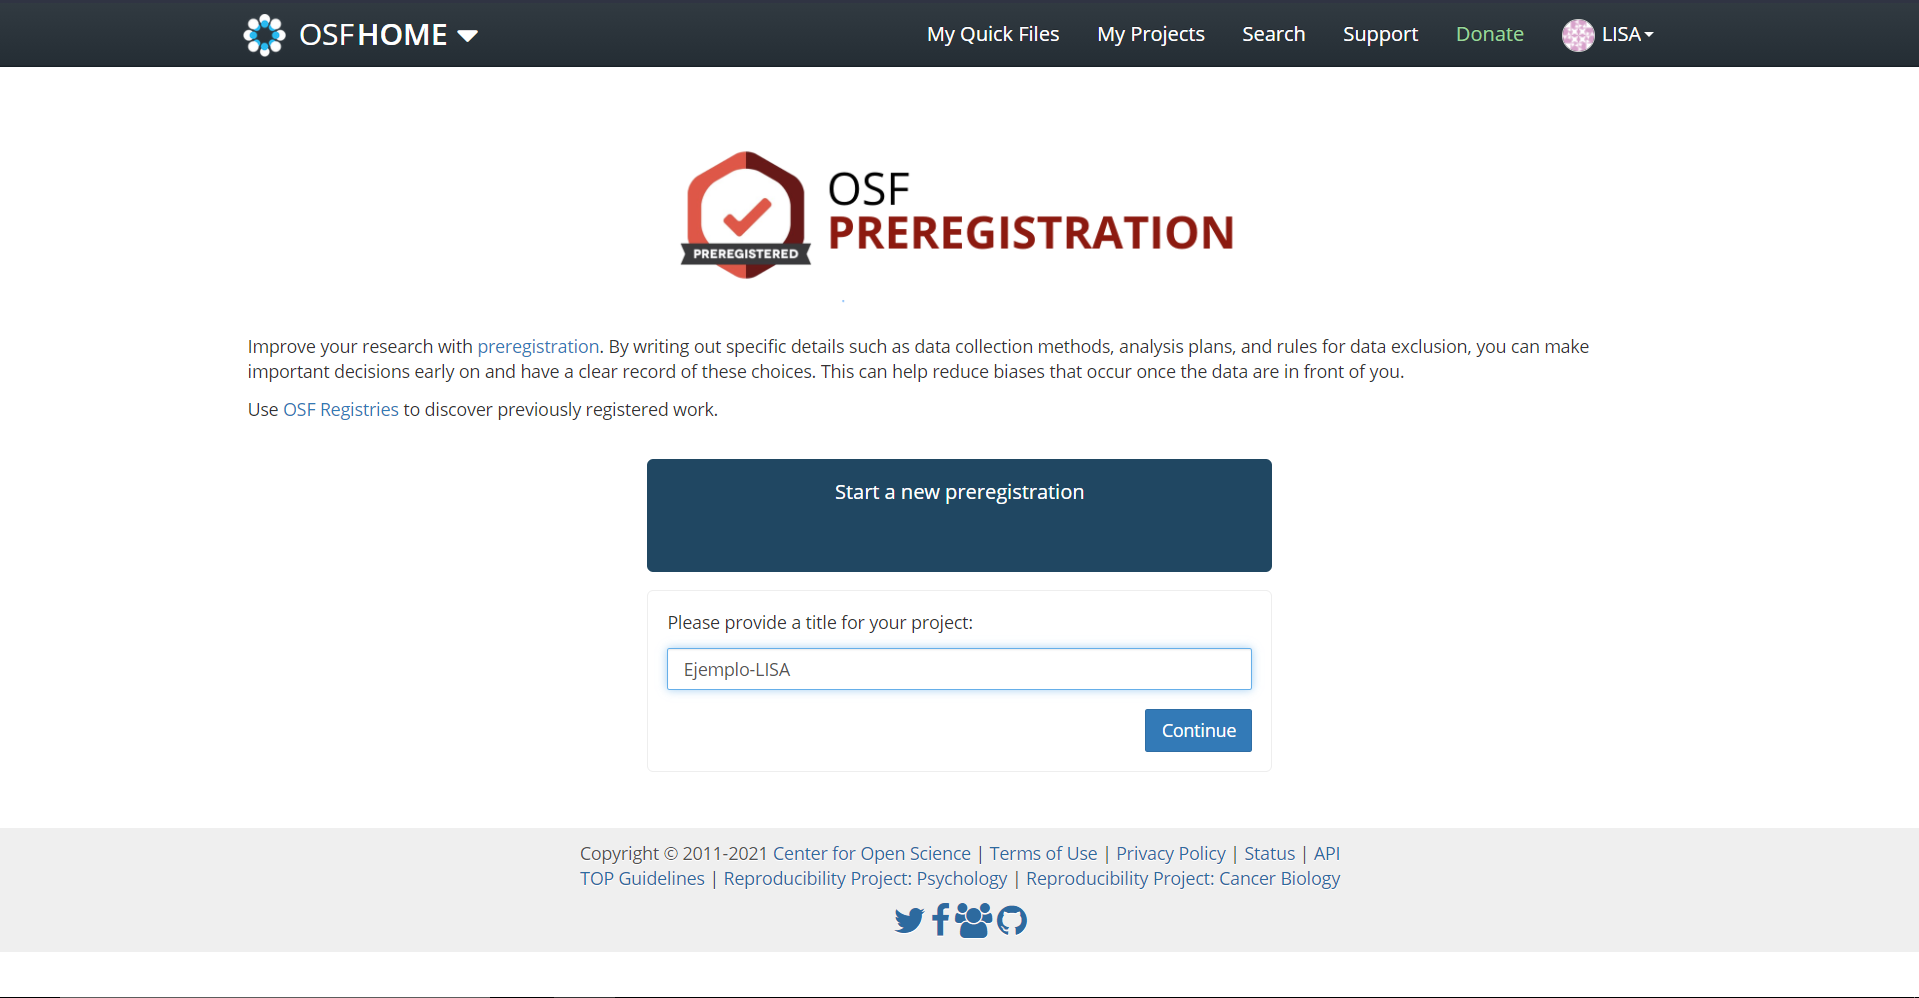
\includegraphics[width=1\linewidth]{docs/images/osfprereg1} 

}

\caption{Preregistros en OSF}\label{fig:osfprereg1}
\end{figure}

\begin{figure}[H]

{\centering 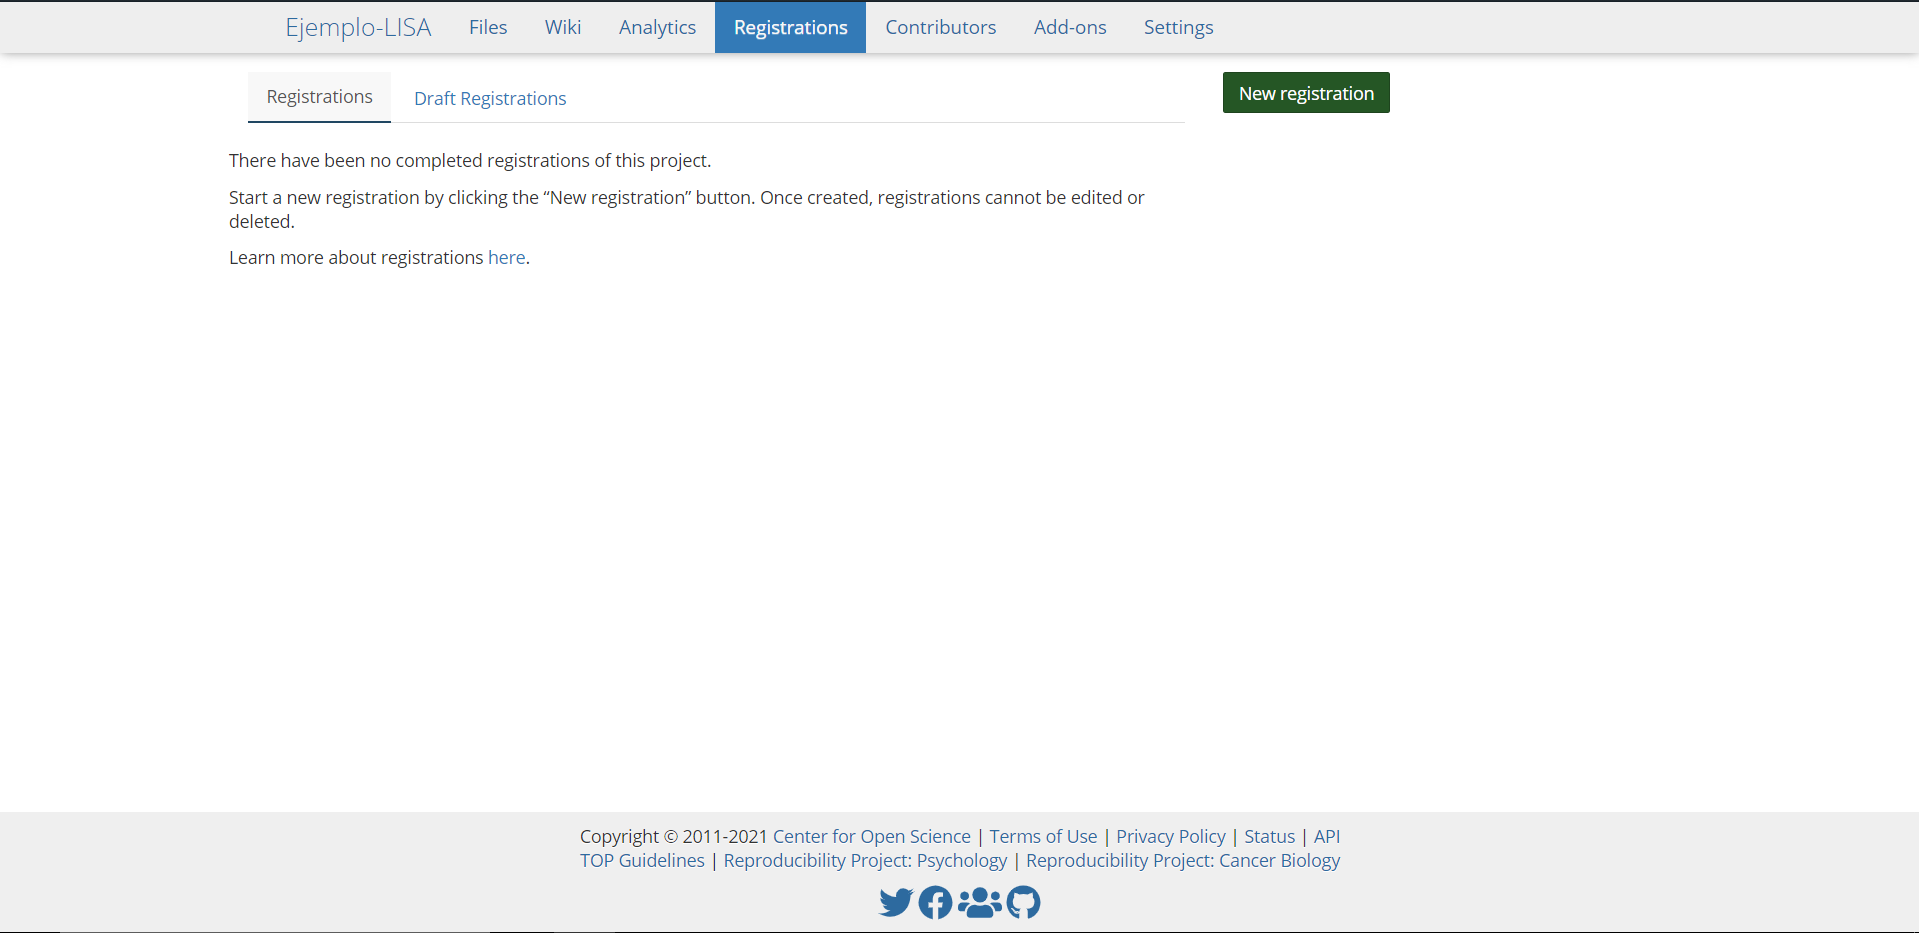
\includegraphics[width=1\linewidth]{docs/images/osfprereg2} 

}

\caption{Preregistros en OSF}\label{fig:osfprereg2}
\end{figure}

En la Figura N° \ref{fig:osfprereg3} podemos ver dos cosas. Primero, la descripción de lo que está haciendo OSF al comenzar un nuevo preregistro, lo que en pocas palabras es una versión no modificable del proyecto al momento que hacemos el preregistro. Tal y como dice la página es una versión ``congelada''. En segundo lugar, también se aprecia una serie de opciones para preregistrar, estas son las plantillas de las que habíamos hablado anteriormente. OSF nos ofrece distintas plantillas de acuerdo al carácter que tiene nuestro estudio. Una breve descripción de cada una es la siguiente:

\begin{itemize}
\item
  OSF Preregistration: Es la plantilla estándar, en la cual se hacen una serie de preguntas relativas al muestreo, diseño y planes de análisis.
\item
  Open-Ended Registration: Consiste en una síntesis narrativa de la investigación a preregistrar. No hay un minimo de palabras para el documento.
\item
  Qualitative Preregistration: Plantilla elaborada por la comunidad de investigadores cualitativos para preregistrar estudios cualitativos.
\item
  Secondary Data Preregistration: También consiste en una serie de preguntas relativas al muestro, diseño y planes de análisis, con algunas pequeñas variaciones.
\item
  Registered Report Protocol Preregistration: Hace unas cuantas preguntas relativas al estudio y permite adjuntar el manuscrito. Esta plantilla se utiliza cuando se está intentando publicar en una revista que adhiere al modelo de Informes Registrados.
\item
  OSF-Standard Pre-Data Collection Registration: Plantilla que sigue el modelo estándar, pero que agrega algunas preguntas más específica sobre recolección de datos. Por ejemplo, pregunta si la recolección de datos está en curso o si se ha hecho algún análisis de los datos hasta ahora.
\item
  Preregistration Template from AsPredicted.org: Plantilla estándarizada de AsPredicted. Simplifica el proceso de preregistro en 9 preguntas clave sobre el estudio.
\item
  Replication Recipe (Brandt et al., 2013): Post-Completion: Se trata de una plantilla para estudios de replicación, especificamente estudios que ya finalizaron.
\item
  Replication Recipe (Brandt et al., 2013): Pre-Registration: Se trata de una plantilla para estudios de replicación que aun no han comenzado.
\item
  Pre-Registration in Social Psychology (van 't Veer \& Giner-Sorolla, 2016): Pre-Registration: Plantilla de preregistro para estudios específicamente de la subdisciplina Psicología Social.
\end{itemize}

\begin{figure}[H]

{\centering 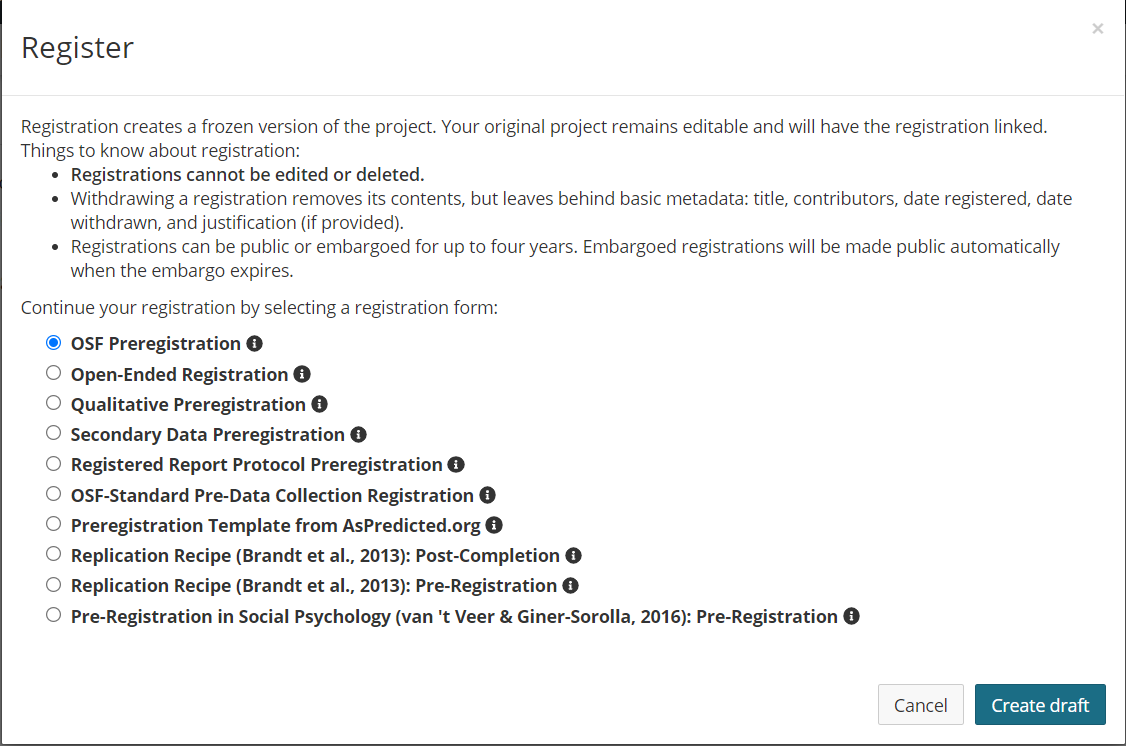
\includegraphics[width=1\linewidth]{docs/images/osfprereg3} 

}

\caption{Preregistros en OSF}\label{fig:osfprereg3}
\end{figure}

\hypertarget{otros}{%
\subsection{Otros}\label{otros}}

\begin{itemize}
\tightlist
\item
  Otras cosas que contribuyen a los preregistros: reporting standards y registered reports
\end{itemize}

\hypertarget{flujos-de-trabajos-reproducibles.}{%
\section{Flujos de trabajos reproducibles.}\label{flujos-de-trabajos-reproducibles.}}

\hypertarget{palabras-finales}{%
\chapter{Palabras finales}\label{palabras-finales}}

Hemos aprendido sobre transparencia y reproducibilidad.

  \bibliography{book.bib,packages.bib}

\end{document}
